\documentclass[xcolor=dvipsnames]{beamer}
\usepackage[utf8]{inputenc}
\usepackage[alf,abnt-repeated-title-omite=yes,abnt-emphasize=bf,abnt-etal-list=0]{abntex2cite}

\usetheme{Madrid}
\usecolortheme{default}

%------------------------------------------------------------
%This block of code defines the information to appear in the
%Title page
\title[Regras Fiscais e Regras Monetárias] %optional
{Unidade 4 - Macroeconomia 1: Política Econômica}

\subtitle{Regras Fiscais e Regras Monetárias}

\author[Luiz Mario, João Rodopoulos] % (optional)
{Luiz Mario, João Rodopoulos}

\institute[ECO-UnB] % (optional)
{
  Departamento de Economia\\
  FACE-UnB
  }

\date[Monitoria 2022] % (optional)
{Monitoria - 1°Semestre de 2022}

\logo{
\includegraphics[height=1cm]{2560px-Webysther_20160322_-_Logo_UnB_(sem_texto).svg.png}}

%End of title page configuration block
%------------------------------------------------------------



%------------------------------------------------------------
%The next block of commands puts the table of contents at the 
%beginning of each section and highlights the current section:

\AtBeginSection[]
{
  \begin{frame}
    \frametitle{Sumário}
    \tableofcontents[currentsection]
  \end{frame}
}
%------------------------------------------------------------


\begin{document}

%The next statement creates the title page.
\frame{\titlepage}


%---------------------------------------------------------
%This block of code is for the table of contents after
%the title page
\begin{frame}
\frametitle{Sumário}
\tableofcontents
\end{frame}
%---------------------------------------------------------


\section{Introdução}

%---------------------------------------------------------
%Changing visivility of the text
\begin{frame}
\frametitle{Introdução - Políticas Econômicas}
Objetivo: alterar a situação econômica presente de um país de acordo com as metas do governo
\begin{itemize}
    \item Metas universais: aumentar renda e emprego, reduzir inflação
\end{itemize}


\end{frame}
%---------------------------------------------------------
\subsection{Tipos de Política Econômica}
%-----------------------------------------------------
\begin{frame}{Política Econômica Ativa x Política Econômica Passiva}
As políticas econômicas podem ser definidas entre ativas e passivas. A definição para tal depende de um análise positiva (influencia dos dados, fatos e modelos) e da análise normativa (Juízos de Valor e visão de mundo do economista) 
\begin{itemize}
    \item Política Econômica Passiva: Visão Liberal (Preços Flexíveis), Auto Regulação do Mercado, Contra intervenções Governamentais. Possui pouca eficácia em períodos de crise. 
    \item Política Economica Ativa: Visão Keynesiana (Preços viscosos ou rígidos),Intervenção do Governo é necessária.  
\end{itemize}
\end{frame}

%---------------------------------------------------------
\begin{frame}{Política Econômica Ativa x Política Econômica Passiva}
Um dos maiores desafios dos policy-makers é perceber qual tipo de política aplicar de acordo com o seu determinado contexto, um dos fatores que mais influenciam isso é a Incerteza.
\begin{itemize}
    \item Muitos dos modelos econométricos e macroeconômicos se baseiam em distribuições de probabilidade, quando conhecemos essa distribuição falamos de risco, quando não conhecemos falamos de incerteza, a postura ativa ou passiva da política econômica é geralmente permeado de incerteza.
    \item Incerteza, em si, significa  na prática que não sabemos a magnitude do efeito dessa política ou a sua duração, se ela ira gerar pontos positivos no futuro ou não, isso se chama efeito encadeamento. 
\end{itemize}

\end{frame}
%--------------------------------------------------------------------
\begin{frame}{Política Econômica Ativa x Política Econômica Passiva}
Existem outros fatores relevantes para a análise como as Expectativas dos agentes e a Crítica de Lucas (os parâmetros não são fixos, estão em constante mudança)
\end{frame}
%---------------------------------------------------------
\subsection{Temporalidade e Hiatos}
%---------------------------------------------------------
\begin{frame}{Temporalidade da Política Econômcia}
Com isso, o impacto de políticas econômicas pode ser definido como uma espécie de "faca de dois gumes",políticas econômicas internas afetam externas e vice e versa, afetando assim o produto, a inflação e o emprego. As reações a essas políticas são definidas por hiatos, sendo eles internos ou externos. 
\begin{itemize}
    \item Hiato Interno: Quanto tempo eu demoro para reagir a uma coisa que aconteceu ? 
    \item Hiato Externo: Agora que eu agi, quanto tempo leva para termos um efeito dessa ação na economia ?
\end{itemize}
\end{frame}
%---------------------------------------------------------
\begin{frame}{Temporalidade da Política Econômcia}
Dentro do debate referente à política fiscal, o hiato interno é maior, dado o rito constitucional necessário para sua aprovação, como por exemplo as leis e regras orçamentárias (LDO, por exemplo). Já na política monetária o hiato interno é no máximo 45 dias, o intervalo de reuniões do COPOM. 
\end{frame}
%---------------------------------------------------------
\subsection{Poder Discrionário e Regras}
%---------------------------------------------------------
%---------------------------------------------------------
\begin{frame}{Poder Discricionário e Regras}
\begin{itemize}
    \item O que significa a política ter regras ? 
    
    Regras trazem compromisso, transparência, credibilidade, previsibilidade e consistência. Mostrando assim a possibilidade de reduzir o hiato interno, porém existem algumas críticas como: Regras feitas sob parâmetros não constantes podem não fazer sentido no futuro, pois elas devem ser revistas e possuir essa flexibilidade
    \item O que significa a política ser livre (Poder Discricionário) ? 
    
    Ser livre possibilita uma maior flexibilidade, levando a avaliação e a tomada de decisão para cada momento específico. Porém, existem algumas críticas: Poder enorme para as pessoas que não são qualificadas, podem ser inconsistentes no aspecto temporal e abrindo a brecha para uma maior interferência política. 
\end{itemize}
    
\end{frame}
%---------------------------------------------------------
%---------------------------------------------------------
%---------------------------------------------------------
%---------------------------------------------------------

\section{Política Fiscal}
%---------------------------------------------------------
\subsection{Definição}
%---------------------------------------------------------
\begin{frame}{Definição de Política Fiscal}
Política fiscal se refere, principalmente, em relação a receitas (arrecadação) e gastos do governo. A receita do governo se da principalmente por meio de tributos, que podem ser divididos em dois grupos: 

\begin{itemize}
    \item Diretos: Sob renda e propriedade (Imposto de Renda, IPVA)
    \item Indiretos: Sob consumo e produção (ICMS,IPI)
\end{itemize}
\end{frame}
%---------------------------------------------------------
\begin{frame}{Definição de Política Fiscal}
No Brasil, os tributos arrecadados são indiretos, recaindo "igualmente" entre ricos e pobres.
Já os gastos podem ser descritos como: 
\begin{itemize}
    \item De Capital: Investimento do Governo 
    \item Correntes: Existem 3 subtipos: Consumo,transferência e financeiro. 
\end{itemize}
O Consumo se refere principalmente à manutenção da máquina pública e salários. Já as transferências se referem a benefícios sociais e aposentadorias e por fim, o financeiro se refere a juros da dívida pública. 
Os gastos correntes são frequentemente criticados pois não aumentam o crescimento no Longo-Prazo.
\end{frame}
%---------------------------------------------------------

\subsection{Curva de Lafer}
%---------------------------------------------------------
\begin{frame}{Curva de Lafer}
A curva de Lafer, basicamente, expoê que existe um limite para a arrecadação de impostos. 
\begin{figure}
    \centering
    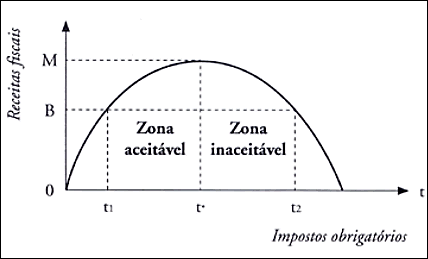
\includegraphics[width=0.70\textwidth]{84c4cf1024e60fe5773b5d4ef2615d8b.png}
    \caption{Curva de Lafer}
    \label{fig:my_label}
\end{figure}
\end{frame}
%---------------------------------------------------------
\begin{frame}{Curva de Lafer}
Por essa curva podemos perceber que caso ocorra um aumento muito grande de impostos, pode haver uma evasão fiscal, levando a uma maior informalidade.
\begin{itemize}
    \item Efeito Renda: O imposto aumentando e a pessoa fica mais pobre, trabalhando mais para compensar e a arrecadação aumenta. 
    \item Efeito Substituição: Quanto maior a alíquota de imposto, uma hora trabalhada a mais gera uma renda que não vale a pena trabalhar para. 
\end{itemize}
Na parte crescente, temos um domínio do efeito renda sob o efeito substituição, o contrário ocorre na parte decrescente. 
\end{frame}
%---------------------------------------------------------
\subsection{Indicadores Fiscais}
%---------------------------------------------------------
\begin{frame}{Indicadores Fiscais}
\begin{itemize}
    \item Indicadores de Fluxo: Défict/Superávit Orçamentário, arrecadação vs gastos em um período. 
    \item Indicadores de Estoque: Dívida 
    \begin{equation}
        D_{t} = (1+i)D_{t-1} - T_{t} + G_{t}
    \end{equation}
\end{itemize}
Somatório de déficts acumulado de fluxos do passado
\end{frame}
%--------------------------------------------------------
\begin{frame}{Indicadores Fiscais}
\begin{itemize}
     \item Resultado Primário:
    \begin{equation}
        RP = T_{t} - G_{t}
    \end{equation}
    Estatística de fluxo para um ano, no período $t$
    Receitas ($T$) - Gastos($G$), excluindo receitas e gastos financeiros 
    \item Resultado Nominal, é o Resultado Primário incluindo gastos e receitas financeiras
    \begin{equation}
        RN = (T_{t} - G_{t}) - iD_{t-1}
    \end{equation}
\end{itemize}
\end{frame}
%---------------------------------------------------------
\begin{frame}{Sobre a Dívida}
A dívida depende de 3 aspectos fundamentais:
\begin{itemize}
    \item Taxa de juros média que inside nela 
    \item Estoque de dívidas já existentes no passado
    \item Resultado Primário 
\end{itemize}
Diminuição de Parte da Dívida é atrelada ao câmbio, melhora de perfil em pré-fixação mostram melhoras na dívida mas ainda é muito grande. Também há de ser ressaltado que a relação dívida-PIB pode dar uma falsa impressão de como o país esta, negligenciando o prazo de pagamento e custo médio da dívida. 
Já o Risco País é o número de pontos percentuais de juros que o país deve pagar em relação a taxa de juros americana (FED) para ser compensado do risco de investir naquele país. 
\end{frame}
%---------------------------------------------------------
\subsection{Regras Fiscais}
%---------------------------------------------------------
\begin{frame}{O que são Regras Fiscais ?}
Podemos definir Regras Fiscais como um mecanismo que introduz, por um certo período de tempo, limites quantitavios para alguma das principais variáveis fiscais de um país, 
De acordo com \cite{Giambiagi}, de forma a conter o viés deficitário do setor público. 
A razão para a existência desse viés deficitário, pode ser também explicada por \cite{Giambiagi}, no seguinte trecho do capítulo "Teto de Gastos: O que aconteceu ?" da seu livro "Tudo sobre o défict público: O Brasil na encruzilhada fiscal".
    
\end{frame}
%---------------------------------------------------------
\begin{frame}{Qual a razão para a natureza deficitária do setor público ?}
"A existência desse viés tem diferentes explicações na literatura. A primeira decorre da informação limitada dos agentes econômicos: como muitos desses não enxergam perfeitamente a restrição orçamentária do governo, tendem a superestimar os benefícios dos gastos correntes e subestimar os custos fiscais a ele associados. Uma segunda explicação associa o viés deficitário com ambientes da acirrada competição política. Nesses casos, a dívida pública pode ser usada estrategicamente pelo governante ara influenciar a escolha de seu sucessor. Outra explicação é relacionada a grupos de pressão. Supondo uma sociedade com diferentes grupos que se beneficiam de determinados tipos de gasto, o governo pode ser influenciado pelo lobby desses grupos, levando a um nível orçamentário maior que o desejado." \cite{Giambiagi}
    
\end{frame}
%---------------------------------------------------------
\subsection{Porque Política Fiscal importa ?}
%---------------------------------------------------------
\begin{frame}{A importância da Política Fiscal}
Porque Política Fiscal importa ? podemos responder isso com base nos seguintes itens:
\begin{itemize}
    \item Diminui a inflação e a fuga de capitais
    \item Traz credibilidade e transparência para o orçamento (isso é um dos principios orçamentários) 
    \item Diminui o viés inflacionário
\end{itemize}
    
\end{frame}
%---------------------------------------------------------
\subsection{Ter Dívida é algo ruim ?}
%---------------------------------------------------------
\begin{frame}{Ter dívida é algo ruim ?}
A reposta é: Não necessariamente, pois:
\begin{itemize}
    \item Ela pode fazer possíveis escolhas intertemporais ótimas, permite atender a situações emergenciais, permite a estabilização automática, pois é contracíclica e diminui o ciclo, pode agir como um controlador da alíquota de imposto.
    \item O grande X da questão é que ela não pode crescer de forma instável!!!!!
\end{itemize}
    
\end{frame}

%---------------------------------------------------------
\subsection{Teto de Gastos}
%---------------------------------------------------------
\begin{frame}{Teto de Gastos}
Regra Fiscal adotada no final de 2016, válida por até 20 anos e se aplica a 3 esferas distintas do Governo Federal, sendo assim limites individualizados para cada órgão. 
Existem exceções para o Teto, gastos eleitorais não entram nele, investimentos em gastos de capital também não entram. 
\end{frame}
%---------------------------------------------------------
\begin{frame}{Equivalência Ricardiana}
 Equivalência ricardiana possui como pressuposto básico que o consumidor se importa com o consumo no período corrente (hoje) e no período posterior a ele (amanhã). O consumidor racional, sabe que dado uma queda na arrecadação tributária hoje é equivalente a mais impostos no futuro.Trazendo isso para uma interpretação mais macro, isso indica que o aumento das despesas do Governo ou corte nos impostos não gera aumento da demanda agregada no curto-prazo.
 Essa ideia possui duas principais críticas:
 \begin{itemize}
     \item Uma relacionada a racionalidade dos agentes, dado que eles podem não ser 100$\%$ racionais a todo tempo, podendo ser miopes.
     \item Keynes: "um aumento dos gastos governamentais pode sim aumentar o nivel de demanda agregada por causa do efeito multiplicador."
 \end{itemize}
    
\end{frame}
%---------------------------------------------------------
\section{Política Monetária}
%---------------------------------------------------------
\subsection{Regras Monetárias}
%---------------------------------------------------------
\begin{frame}{Regras Monetárias - Introdução}
Como dito no início, a política monetária é um instrumento da política econômica utilizado para estabilizar a economia. Ela impacta a economia afetando o custo do dinheiro, por meio do controle da taxa básica de juros, essa taxa pode afetar a inflação futura da economia, e outra execução de política econômica é o controle da quantidade de moeda em circulação na economia. Isso pode ser feito por uma alteração na taxa de recolhimento compulsório, operações com títulos públicos ou emitindo uma maior/menor quantidade de moeda. 
\end{frame}
%---------------------------------------------------------
%---------------------------------------------------------
%---------------------------------------------------------
%---------------------------------------------------------
\subsection{Regra de Taylor}
%---------------------------------------------------------
\begin{frame}{Regra de Taylor - Definição}
    
O instrumento de política monetária principal que será analisado é a fixação da taxa básica de juros. Essa manipulação da taxa básica de juros é importante para manter a inflação em patamares baixos, o que é uma das metas universais de política econômica. A suposição de que o nível da taxa de juros teria impacto no nível da taxa de juros vem da Regra de Taylor. 

A Regra de Taylor é uma equação que relaciona a taxa básica de juros com o nível de inflação e o hiato do produto (diferença entre PIB potencial e PIB real) de um país. Com ela, em teoria, o banco central pode descobrir qual a taxa básica de juros necessária para chegar à meta desejada para a inflação em um período futuro.
\end{frame}
%---------------------------------------------------------
\begin{frame}[t]
\frametitle{Regra de Taylor - Equação}
\begin{alertblock}{Regra de Taylor}
\begin{equation}
    i - i^{*} = \alpha_{\pi}(\pi - \pi^{*}) + \alpha_{y}(Y - Y^{*})
\end{equation}
\end{alertblock}
Em que:
\begin{itemize}
    \item $i$ é a taxa de juros real e $i^{*}$ é a taxa de juros real de equilíbrio
    \item $\alpha_{\pi}$ é o coeficiente de sensibilidade à variação da inflação
    \item $\pi$ é a taxa de inflação anual observada e $\pi^{*}$ é a meta de inflação
    \item $\alpha_{y}$ é o coeficiente de sensibilidade à variação do produto 
    \item $Y$ é o Produto Interno Bruto (PIB) e $Y^{*}$ é o PIB de pleno emprego dos fatores de produção. Podemos definir também $Y - Y^{*}$ como hiato do produto.
\end{itemize}
\end{frame}
%--------------------------------------------
\subsection{Regime de Metas para Inflação}
%--------------------------------------------
\begin{frame}{Regime de Metas}
O Regime de Metas para Inflação é uma política econômica na qual o Banco Central de um país estabelece uma meta para o nível de inflação em um determinado período e se compromete a usar os instrumentos que tiver para alcançar essa meta. Os instrumentos principais utilizados são a manipulação da taxa de juros, da taxa de câmbio, expansão/redução da base monetária. O Banco Central anuncia uma meta, ao início de um período, se responsabiliza por atingir essa meta e torna a comunicação com o público mais transparente sobre o processo para cumprir a meta, buscando um retorno positivo das expectativas dos agentes econômicos. As expectativas dos agentes dentro de uma economia possuem um papel fundamental na eficiência de políticas econômicas.
    
\end{frame}
%--------------------------------------------. 
\begin{frame}{Regime de Metas}
No caso desse regime, a credibilidade possui um papel muito importante no desempenho do Banco Central para alcançar a meta. Se o BC se mostra comprometido em atingir a meta estabelecida, utilizando os instrumentos que possui de forma condizente com o objetivo, ele transmitirá maior credibilidade para a população, o que afeta positivamente as expectativas dos agentes da economia. Caso o BC mostre que não está usando os instrumentos de forma adequada para atingir a meta, não honrando com seu compromisso, ele perderá sua credibilidade com a população, o que afeta negativamente as expectativas dos agentes da economia e dificulta mais ainda o cumprimento da meta inflacionária. 
O BC se utiliza da Regra de Taylor para o controle inflacionário, se relacionando com o regime de metas.
    
\end{frame}
%--------------------------------------------
\begin{frame}{Regime de Metas}
No caso do Brasil, o Regime de Metas usa como referência para o nível de inflação o IPCA (Índice de Preços do Consumidor Amplo). Por meio desse índice, o Banco Central avalia o funcionamento das suas políticas para atingir o nível de inflação desejado ao final do período. Segundo o próprio Banco Central brasileiro, o regime de metas brasileiro envolve: conhecimento público e prévio da meta, autonomia do banco central na adoção de medidas necessárias para atingir a meta, comunicação transparente e regular sobre os objetivos e justificativas das decisões da política monetária e mecanismos de incentivo e responsabilização para que o Banco Central cumpra a meta.
    
\end{frame}
%--------------------------------------------
\begin{frame}{Regime de Metas}
O Banco Central brasileiro possui uma “taxa de tolerância” para essa meta, ou seja, existe uma faixa de valores para a inflação acima e abaixo da meta fixada que ainda é considerada aceitável e dentro da meta. Em 2021, a meta para a inflação do ano era de 3,75$\%$ a.a. com uma margem de tolerância de 1,5$\%$ para mais ou para menos, e a inflação foi de 10,06$\%$, estando, portanto, fora da meta. Quando casos como esse ocorrem, de a meta não ter sido cumprida, representantes do Banco Central devem ir a público prestar esclarecimentos sobre o porquê não foi possível atingir a meta estipulada.
    
\end{frame}
%--------------------------------------------
\begin{frame}{Regime de Metas}
\begin{figure}
    \centering
    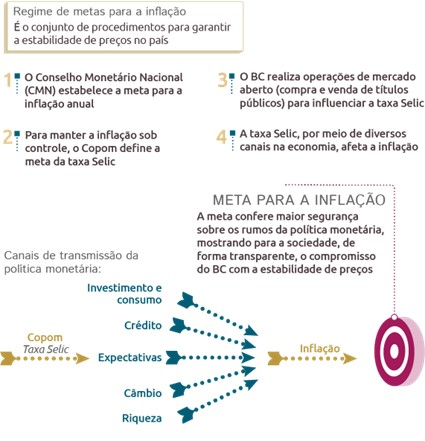
\includegraphics[width=0.70\textwidth]{Figuras/metasinflacao.jpg}
    \caption{Mapa Mental do Regime de Metas}
    \label{fig:my_label}
\end{figure}
    
\end{frame}
%--------------------------------------------
\begin{frame}{Regime de Metas}
\begin{figure}
    \centering
    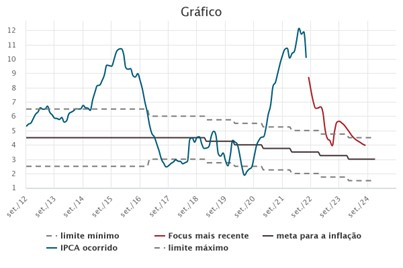
\includegraphics[width=0.70\textwidth]{Figuras/graficomonetaria.jpg}
    \caption{}
    \label{fig:my_label}
\end{figure}
    
\end{frame}
%--------------------------------------------

\section{Referências}
%--------------------------------------------
\begin{frame}{Referências Bibliográficas}
\renewcommand{\refname}{}
\bibliography{bib}
\end{frame}

\end{document}